\documentclass{standalone}
\usepackage{tikz}
\usepackage{amsmath}
\usepackage{amssymb}
\usepackage{mathrsfs}

\begin{document}

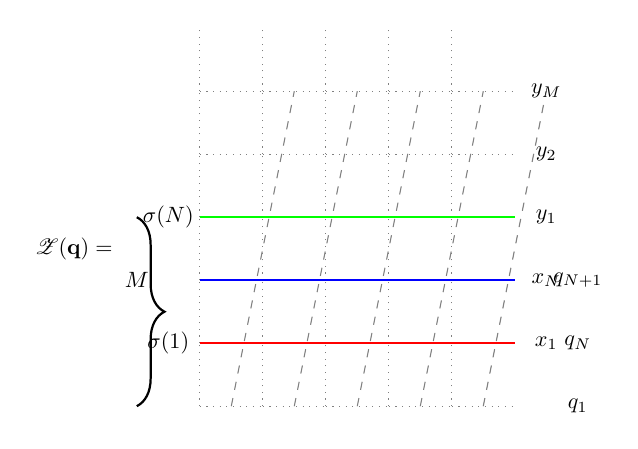
\begin{tikzpicture}[scale=0.8, every node/.style={scale=0.8}]

% Dotted grid
\foreach \i in {0,1,...,4} {
    \foreach \j in {0,1,...,5} {
        \draw[gray, dotted] (\i, \j) -- (\i+1, \j);
    }
}

\foreach \j in {0,1,...,5} {
    \foreach \i in {0,1,...,4} {
        \draw[gray, dotted] (\i, \j) -- (\i, \j+1);
    }
}

% Horizontal lines
\draw[thick, red] (0,1) -- (5,1);
\draw[thick, blue] (0,2) -- (5,2);
\draw[thick, green] (0,3) -- (5,3);

% Diagonal lines crossing
\foreach \i in {0,1,...,4} {
    \draw[gray, dashed] (\i+0.5, 0) -- (\i+1.5, 5);
}

% Labels
\node at (-0.5, 3) {$\sigma(N)$};
\node at (-0.5, 1) {$\sigma(1)$};
\node at (-1, 2) {$M$};

% q and x labels
\node at (5.5, 5) {$y_M$};
\node at (5.5, 4) {$y_2$};
\node at (5.5, 3) {$y_1$};

\node at (6, 2) {$q_{N+1}$};
\node at (6, 1) {$q_N$};
\node at (6, 0) {$q_1$};

\node at (5.5, 2) {$x_N$};
\node at (5.5, 1) {$x_1$};

% Curly brace
\draw[decorate, decoration={brace, amplitude=10pt, mirror}, thick] (-1, 0) -- (-1, 3) node[midway,xshift=-10pt] {};

% Equation label
\node at (-2, 2.5) {$\mathscr{Z}(\mathbf{q}) = $};

\end{tikzpicture}

\end{document}